\part{Wissensrepräsentation und lineare kontinuierliche Systeme}
\section{Wissen}
\subsection{Modellbildung}
\subsubsection{}
\textbf{Welche zwei Eebenen der Modellbildung sind Ihnen aus der Vorlesung bekannt? Nennen Sie jeweils ein Beispiel für ein solche Modell.}

Diskrete ereignisorientierte Modelle und Räumlich-Zeitliche Modelle:
\begin{figure}[H]
    \centering
    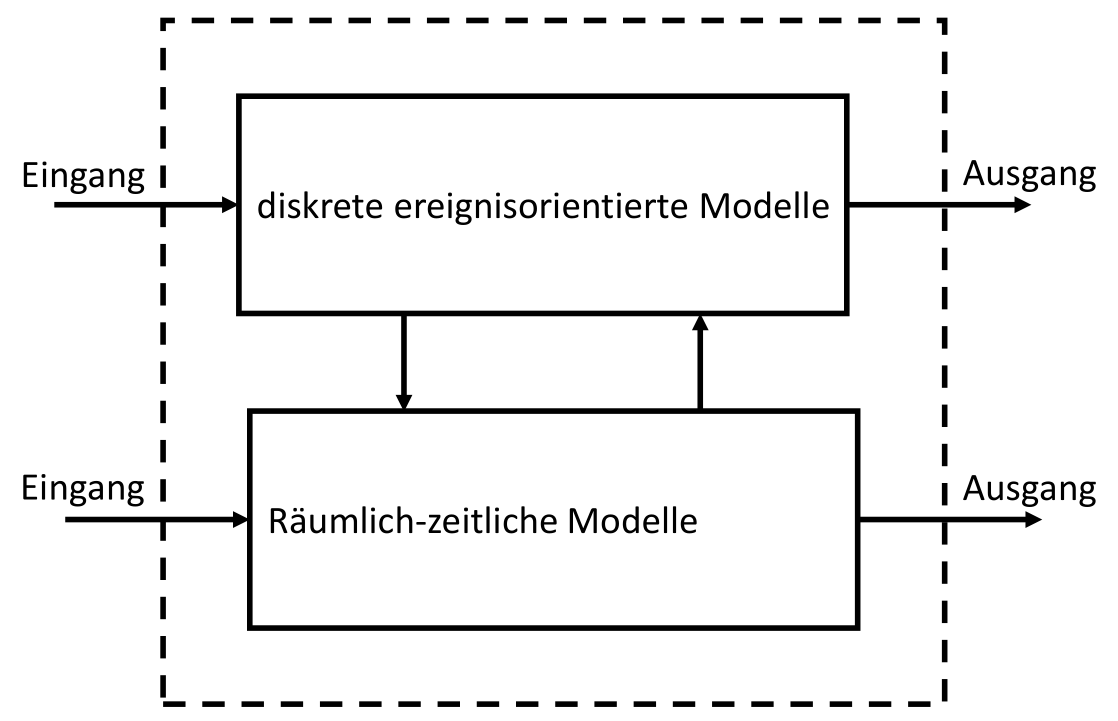
\includegraphics[width=.4\linewidth]{Graphics/Modellbildung_Ebenen.png}
    \caption{Unterschiedliche Beschreibungsebenen}
\end{figure}
\begin{figure}[H]
    \centering
    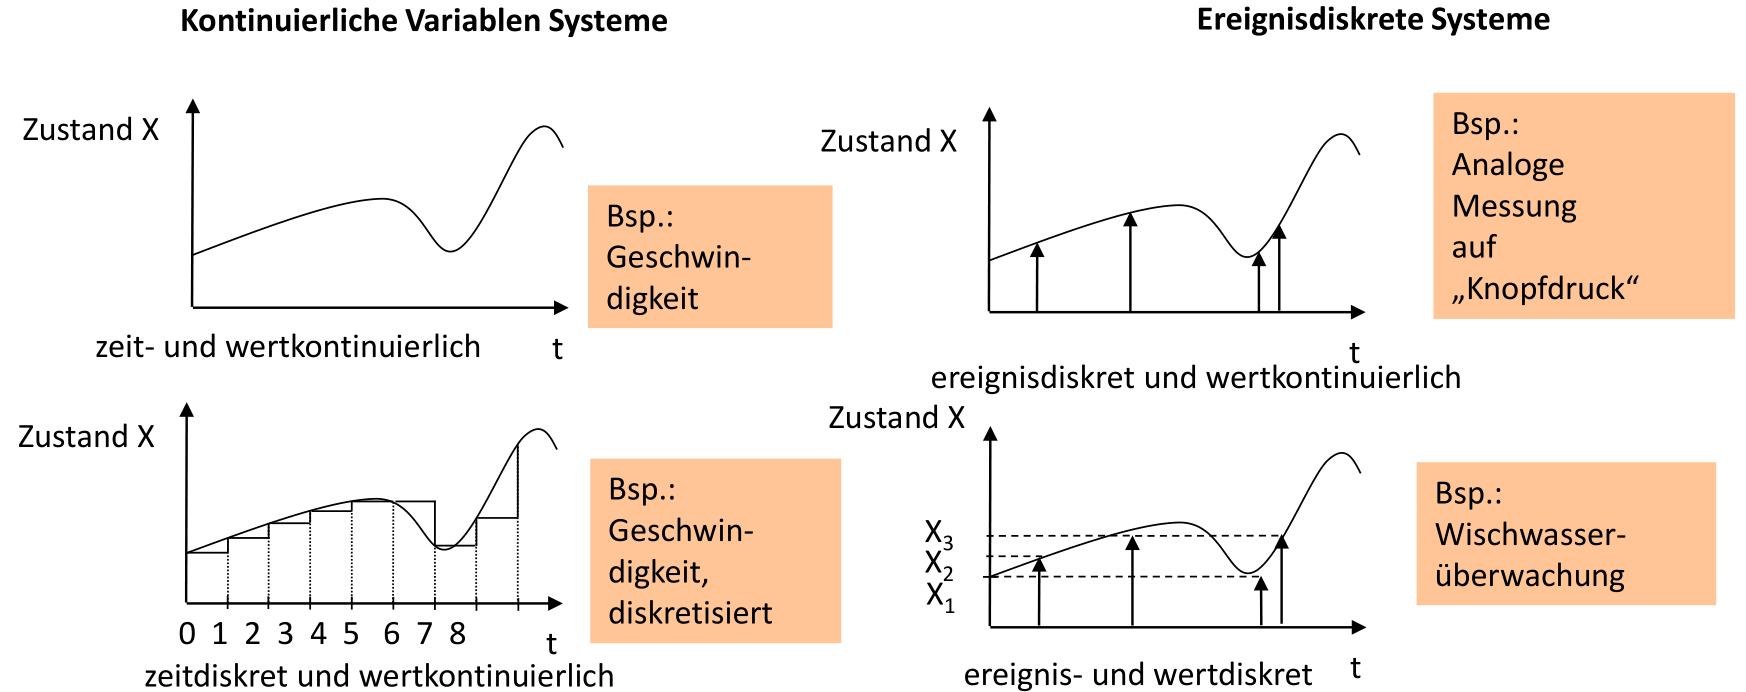
\includegraphics[width=.6\linewidth]{Graphics/Beispiel_Modell.png}
    \caption{Beispiele}
\end{figure}

\subsection{Querführungsmodell}
\subsubsection{}
\textbf{Sie haben in der Vorlesung das Querführungsmodell 5. Ordnung kennengelernt. Wie unterscheidet sich dieses qualitativ vom Einspurmodell?}
\begin{itemize}
    \item Einspurmodell beschreibt Fahrzeugbewegung im freien Raum
    \item Reglung von Fahrzeugen im Fahrstreifen für Fahrfunktionen relevant
    \item Querführungsmodell integriert Fahrbahnrelation in das Modell
\end{itemize}

\subsubsection{}
\textbf{Was versteht man qualitativ unter dem Begriff der Steuerbarkeit?(hier ist kein mathematisches Kriterium gefragt)}

Sollte es Komponenten des Zustandsvektor $x(t)$ des Systems, die nicht vom Eingangsvektor $u(t)$ beeinflusst werden geben, dann wäre es naheliegend, das system als nicht steuerbar zu bezeichnen.

Ein lineares System ist vollständig zustandssteuerbar, wenn es für jeden Anfangszustand x(t0) eine Steuerfunktion u(t) gibt, die das System innerhalb einer beliebigen Zeitspanne $t_0 < t < t_1$ in den Endzustand x(t1)=0 überführt.

\subsubsection{}
\textbf{Was versteht man qualitativ unter dem Begriff der Beobachtbarkeit?(hier ist kein mathematisches Kriterium gefragt)}

Sollte es Komponenten des Zustandsvektors $x(t)$ des Systems, die keine Einfluss auf den Ausgangsvektor $y(t)$ ausüben geben, dann kann aus dem Verhalten des Ausgangsvektors $y(t)$ nicht auf den Zustandsvektor $x(t)$ geschlossen werden, und es liegt nahe, das betreffende System als nicht beobachtbar zu bezeichnen.

Ein lineares System ist vollständig beobachtbar, wenn man bei bekannter äußerer Beeinflussung Bu(t) und bekannten Matrizen A und C aus dem Ausgangsvektor y(t) über ein endliches Zeitintervall $t_0 < t < t_1$ den Anfangszustand x(t0) eindeutig bestimmen kann.

\subsection{Beobachter}
\subsubsection{}
\textbf{Was ist die Grundidee, die hinter einem Beobachter steckt? (hier ist kein mathematisches Kriterium gefragt)}

\begin{figure}[H]
    \centering
    \begin{minipage}{.45\linewidth}
        \begin{itemize}
            \item Interne Nachbildung der Regelstrecke
            \item Vorsicht: Anfangsvektor $x(t_0)$ nicht bekannt!
        \end{itemize}
    \end{minipage}
    \begin{minipage}{.5\linewidth}
        \centering
        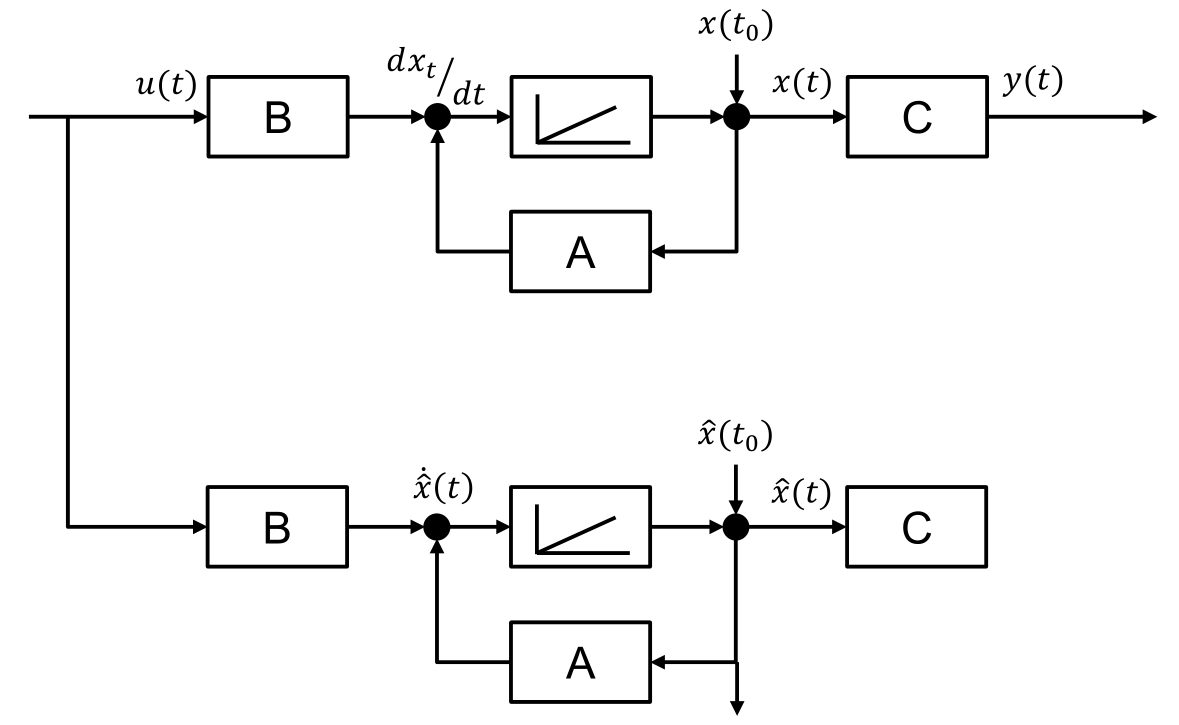
\includegraphics[width=.99\linewidth]{Graphics/Beobachter_Grundidee.png}
    \end{minipage}
\end{figure}

\subsection{Ereignisdiskrete Systeme}
\subsubsection{}
\textbf{Wodurch zeichnen sich ereignisdiskrete Systeme aus?}

\begin{figure}[H]
    \centering
    \begin{minipage}{.4\linewidth}
        \begin{itemize}
            \item X: Menge von Eingangsvariablen
            \item Y: Menge der Ausgangsvariablen
            \item Z: Zustandsvariablen/Zustände
            \item $\Phi()$: Übergangsfunktion bestimmt den Zustandsübergang aufgrund der Eingabe oder des Zeitverlaufs
            \item $\Omega()$: Ausgabefunktion bestimmt die Ausgaben aufgrund der Zustandsübergänge
        \end{itemize}
    \end{minipage}
    \begin{minipage}{.5\linewidth}
        \centering
        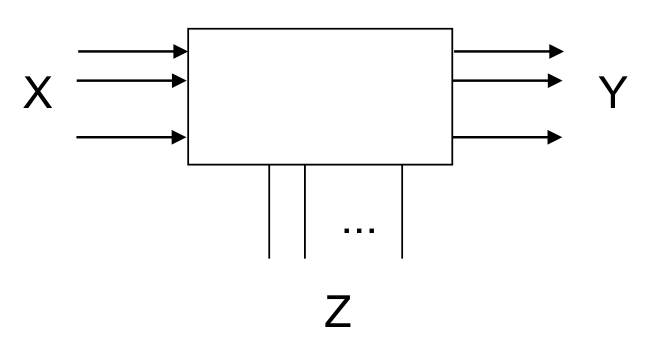
\includegraphics[width=.99\linewidth]{Graphics/Ereignisdiskrete_Systeme.png}
    \end{minipage}
\end{figure}

\subsubsection{}
\textbf{In der Vorlesung haben Sie Automanten als Form der Modellierung ereignisdiskreter Systeme kennengelernt. Was zeichnet einen Moore-Automaten aus? Was einen Mealy-Automaten?}

\textbf{Geben Sie ein Beispiel f"ur einen Moore- und einen Mealy-Automaten an.}

\begin{figure}[H]
    \centering
    \begin{minipage}{.48\linewidth}
        \centering
        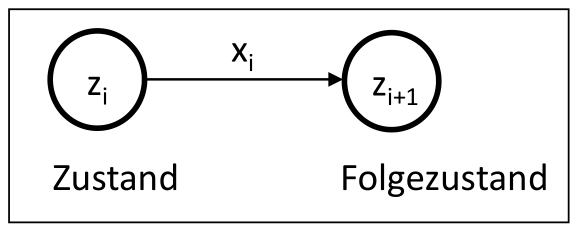
\includegraphics[width=.95\linewidth]{Graphics/Moore_automaten_1.png}
        \caption{Moore-Automaten}
    \end{minipage}
    \begin{minipage}{.48\linewidth}
        \centering
        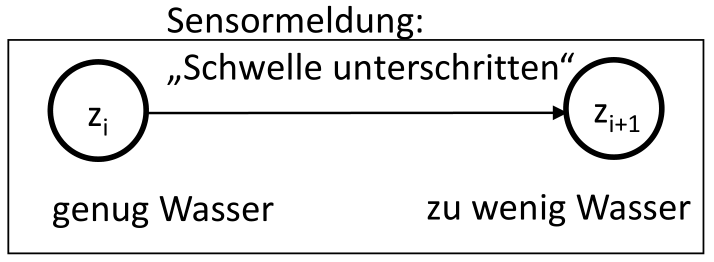
\includegraphics[width=.95\linewidth]{Graphics/Moore_automaten_2.png}
        \caption{Beispiel}
    \end{minipage}
    \begin{minipage}{.48\linewidth}
        \centering
        \includegraphics[width=.95\linewidth]{Graphics/Mealy_automaten_1.png}
        \caption{Mealy-Automaten}
    \end{minipage}
    \begin{minipage}{.48\linewidth}
        \centering
        \includegraphics[width=.95\linewidth]{Graphics/Mealy_automaten_2.png}
        \caption{Beispiel}
    \end{minipage}
\end{figure}

\section{Lineare kontinuierliche Systeme}
\subsection{}
\textbf{Welche Annahmen liegen dem linearen Einspurmodell zugrunde? Nennen Sie mindestens 5 Stück.}
\begin{itemize}
    \item Reduktion auf ein Rad pro Achse, d.h. $s_l=s_r=0;\ c_{\alpha}=c_{\alpha,l}+c_{\alpha_r}$
    \item Gesamte Masse im Schwerpunkt
    \item Schwerpunkt auf Höhe der Fahrbahn (damit Betrachtung von Wank-, Nick-, und Hubbewegung wegfällt)
    \item Konstante Fahrzeuggeschwindigkeit
    \item Kleine Winkel ($\sin x=x, \cos x=1, \tan x=x$)
    \item Keine Radlastschwankungen
    \item Zwei Systemzustände (Gierrate $\dot{\psi}$, Schwimmwinekl $\beta$)
    \item Lineare Reifenkennlinie
    \item Reine Vorderachslenkung $\delta_H=0$
    \item Gültig bis ca. $|a_y|\leq4\dfrac{m}{s^2}$
\end{itemize}

\subsection{}
\textbf{Zeichnen Sie ein Blockschaltbild eines dynamischen Systems mit Beobachter. Beschriften Sie das Blockschaltbild sorgfältig.}
\begin{figure}[H]
    \centering
    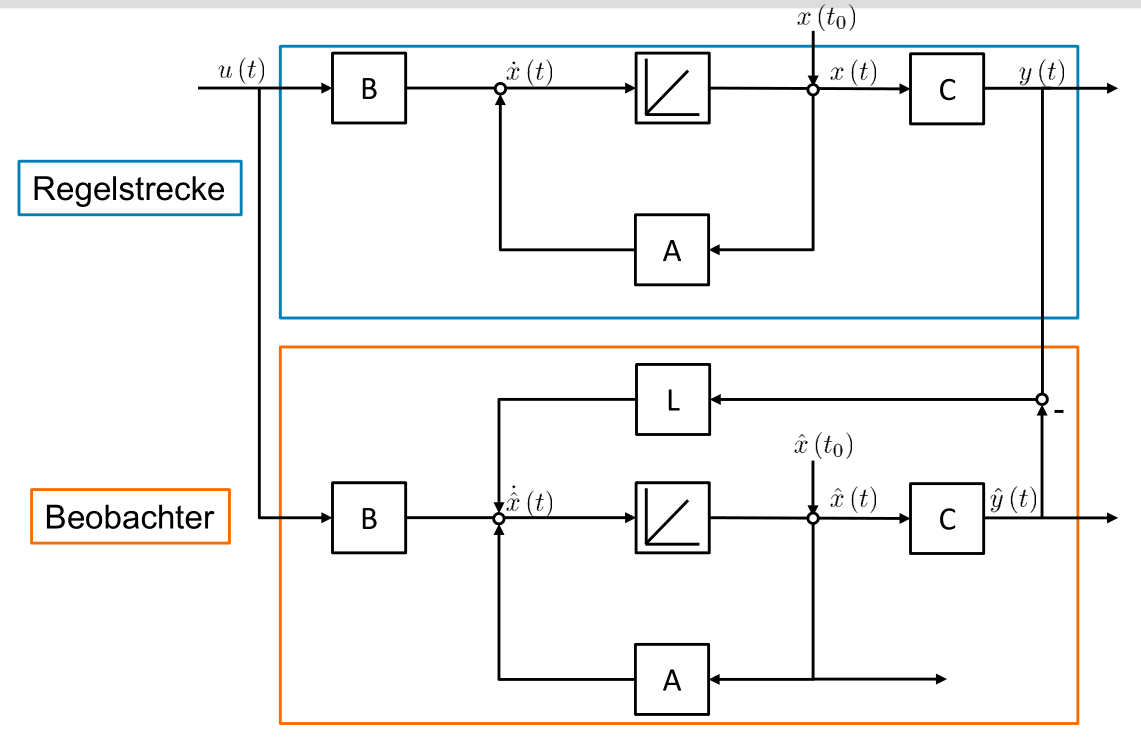
\includegraphics[width=.5\linewidth]{Graphics/beobrachter_blockbild.png}
\end{figure}
\subsection{}
\textbf{Reduzieren Sie das gegebene Querführungsmodell 5.Ordnung soweit wie möglich, so dass damit ein Schwimmwinkelbeobachter konstruierbar ist. Notieren Sie das Modell in Zustandsdarstellung unter der Annahme, dass der Lenkwinkel die einzige Eingangsgröße ist.}

\begin{equation}
    \left(
    \begin{array}{c}
            \dot{\lambda}    \\
            \ddot{\Psi_V}    \\
            \dot{\beta}      \\
            \dot{\Psi_{rel}} \\
            \dot{y}          \\
        \end{array}
    \right)=
    \left(
    \begin{array}{ccccc}
            0                                & 0                                                        & 0                                                   & 0 & 0 \\
            \dfrac{c_{\alpha v}l_{v}}{I_{z}} & -\dfrac{c_{\alpha v}l_{v}^2+c_{\alpha h}l_{h}^2}{I_{z}v} & -\dfrac{c_{\alpha v}l_{v}-c_{\alpha h}l_{h}}{I_{z}} & 0 & 0 \\
            \dfrac{c_{\alpha v}}{mv}         & -1-\dfrac{c_{\alpha v}l_{v}-c_{\alpha h}l_{h}}{mv^2}     & -\dfrac{c_{\alpha v}+c_{\alpha h}}{mv}              & 0 & 0 \\
            0                                & 1                                                        & 0                                                   & 0 & 0 \\
            0                                & 0                                                        & v                                                   & v & 0 \\
        \end{array}
    \right)
    \left(
    \begin{array}{c}
            \lambda      \\
            \dot{\Psi_V} \\
            \beta        \\
            \Psi_{rel}   \\
            y            \\
        \end{array}
    \right)+
    \left(
    \begin{array}{c}
            1 \\
            0 \\
            0 \\
            0 \\
            0 \\
        \end{array}
    \right)\dot{\lambda}+
    \left(
    \begin{array}{c}
            0  \\
            0  \\
            0  \\
            -v \\
            0  \\
        \end{array}
    \right)c_0
\end{equation}

\begin{equation}
    \left(
    \begin{array}{c}
        \ddot{\Psi_V} \\
        \dot{\beta}   \\
    \end{array}
    \right)=
    \left(
    \begin{array}{cc}
        -\dfrac{c_{\alpha v}l_{v}^2+c_{\alpha h}l_{h}^2}{I_{z}v} & -\dfrac{c_{\alpha v}l_{v}-c_{\alpha h}l_{h}}{I_{z}} \\
        -1-\dfrac{c_{\alpha v}l_{v}-c_{\alpha h}l_{h}}{mv^2}     & -\dfrac{c_{\alpha v}+c_{\alpha h}}{mv}              \\
    \end{array}
    \right)
    \left(
    \begin{array}{c}
        \dot{\Psi_V} \\
        \beta        \\
    \end{array}
    \right)+
    \left(
    \begin{array}{c}
        \dfrac{c_{\alpha v}l_v}{I_{Z}} \\
        \dfrac{c_{\alpha v}}{mv}       \\
    \end{array}
    \right)\lambda
\end{equation}

\subsection{}
\textbf{Beschriften Sie folgende schematische Darstellung des linearen Einspurmodells in der nachstehenden Tabelle.}

\begin{figure}[H]
    \centering
    \begin{minipage}[c]{.24\linewidth}
        \centering
        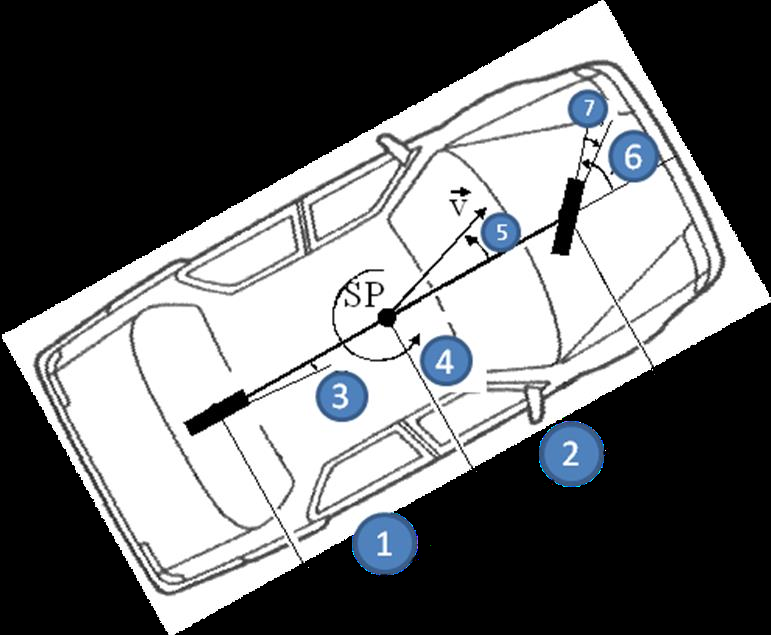
\includegraphics[width=\linewidth]{Graphics/Linearen_Einspurmodell.png}
    \end{minipage}
    \begin{minipage}[c]{.75\linewidth}
        \centering
        \begin{tabular}{|p{.05\linewidth}<{\centering}|p{.115\linewidth}<{\centering}|p{.75\linewidth}<{\centering}|}
            \hline
            Nr. & Bezeichnung & Bedeutung                        \\
            \hline
            1   & $l_H$       & Schwerpunktvorlage               \\
            \hline
            2   & $l_V$       & Schwerpunktr\"ucklage            \\
            \hline
            3   & $\alpha_H$  & Schräglaufwinkel von Hinterachse \\
            \hline
            4   & $\Psi$      & Gierwinkel                       \\
            \hline
            5   & $\beta$     & Schwimmwinkel                    \\
            \hline
            6   & $\delta$    & Lenkwinkel                       \\
            \hline
            7   & $\alpha_V$  & Schräglaufwinkel von Vorderachse \\
            \hline
        \end{tabular}
    \end{minipage}
\end{figure}

\subsection{}
\subsubsection{}
\textbf{Wie ist der Schwimmwinkel im Fahrzeug definiert?}
\begin{figure}[H]
    \centering
    \begin{minipage}{.4\linewidth}
        \centering
        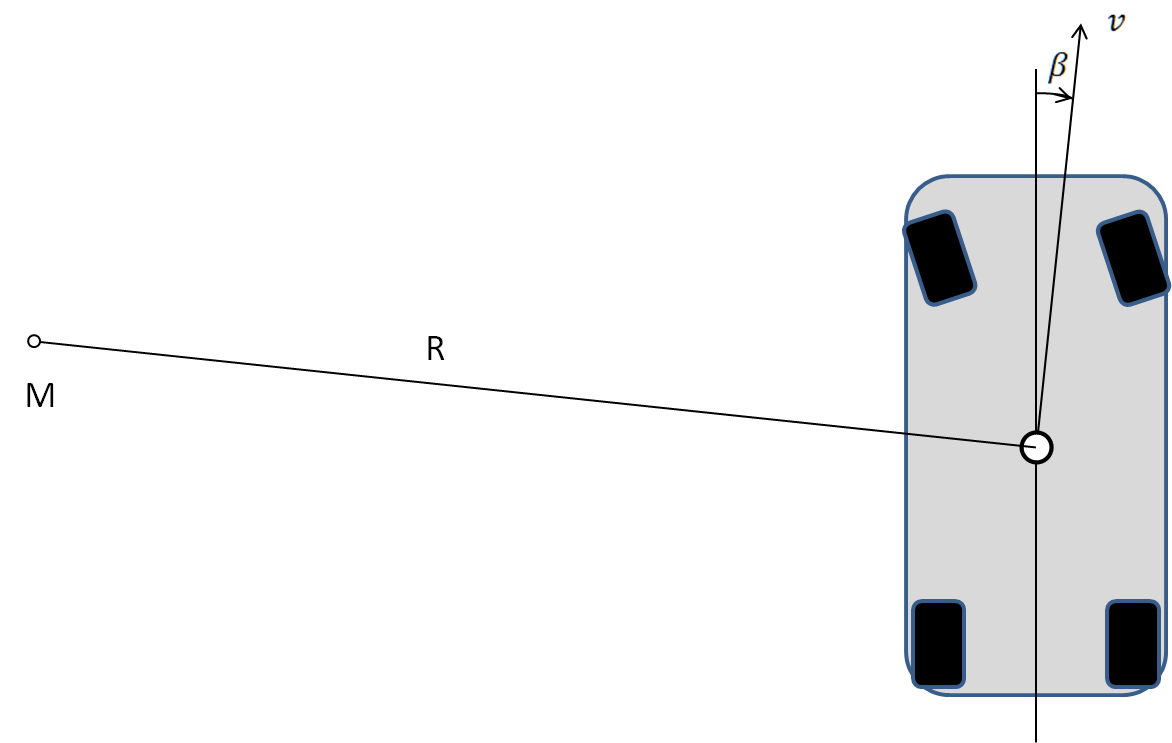
\includegraphics[width=\linewidth]{Graphics/Schwimmwinkel.png}
    \end{minipage}
    \begin{minipage}{.55\linewidth}
        Der Schwimmwinkel ist der Winkel β zwischen der Bewegungsrichtung des Fahrzeugs im Schwerpunkt und der Fahrzeuglängsachse.
    \end{minipage}
\end{figure}
\subsubsection{}
\textbf{Welche Bedeutung hat der Schwimmwinkel bzgl. der Dynamik des Fahrzeugs?}
\begin{equation}
    \begin{aligned}
        a_{y,trans}            & =\dfrac{\dif v_y}{\dif t}                                                               \\
                               & =v\dot{\beta}\underbrace{\cos\beta}_1+\underbrace{\dot{v}\sin\beta}_{0,\ da\ \dot{v}=0} \\
                               & =b\dot{\beta}                                                                           \\                                                                           \\
        a_{y,rot}              & =\dfrac{v^2}{R}\quad mit\ v=\dot{\Psi}R                                                 \\
                               & =\dfrac{v\cdot\overbrace{\dot{\Psi}R}^v}{R}=v\cdot\dot{\Psi}                            \\
        Superposition\quad a_y & =a_{y,trans}+a_{y,rot}                                                                  \\
                               & =v\cdot\left(\dot{\beta}+\dot{\Psi}\right)
    \end{aligned}
\end{equation}

\section{Beobachter}
\subsection{}
\textbf{Wo liegen die Pole der Übertragungsmatrix eines Beobachters in Abhängigkeit von der Rückführungsmatrix L? Geben Sie eine Herleitung für Ihr Ergebnis an.}
\begin{equation}
    \begin{aligned}
        \dot{\hat{x}}               & =A\hat{x}+Bu+L(y-\hat{y})                                                                                               \\
        \hat{y}                     & =c\hat{x}                                                                                                               \\
        \dot{\hat{x}}               & =a\hat{x}+Bu+Ly-LC\hat{x}                                                                                               \\
                                    & =\left(A-LC\right)\hat{x}+Bu+Ly                                                                                         \\
        s\hat{X}                    & =\left(A-LC\right)\hat{X}+Bu+LY                                                                                         \\
        \left(sI-A+LC\right)\hat{X} & =Bu+LY                                                                                                                  \\
        \hat{X}                     & =\textcolor{red}{\underbrace{\left(sI-A+LC\right)^{-1}}_{Polverteilung\ \ddot{U}bertragungsfunktion}}\left(Bu+LY\right) \\
    \end{aligned}
\end{equation}

\subsection{}
\textbf{Für folgendes System soll ein Beobachter zur Zustandsrekonstruktion so entworfen werden, dass die Beobachterfehlerdynamik einen doppelten Pol bei $s=-2$ aufweist.}

\begin{equation}
    \begin{array}{l}
        \dot{x}=\left[\begin{array}{cc}
                2  & 1 \\
                -1 & 0 \\
            \end{array}\right]x+\left[\begin{array}{c}
                0 \\
                1 \\
            \end{array}\right]u \\
        y=\left[1\qquad 0\right]x
    \end{array}
\end{equation}
\subsubsection{}\textbf{Überprüfen Sie das System auf die Beobachtbarkeit.}

Kriterium:
\begin{equation}
    Q_B=\left[\begin{array}{c}
            C  \\
            CA \\
        \end{array}\right]\rightarrow\detmat\ Q_B\neq0
\end{equation}
\begin{equation}
    Q_B=\left[\begin{array}{cc}
            1 & 0 \\
            2 & 1 \\
        \end{array}\right]\rightarrow\detmat\ Q_B=1\rightarrow beobachtbar
\end{equation}
\subsubsection{}\textbf{Bestimmen Sie die Beobachterkoeffizienten $l_1$ und $l_2$.}

\begin{equation}
    \detmat(sI-A+LC)=\left|\left[\begin{array}{cc}
            s-2+l_1 & -1 \\
            1+l_2   & s  \\
        \end{array}\right]\right|=s^2-2s+l_1s+1+l_2
\end{equation}
Weil die Beobachterfehlerdynamik einen doppelten Pol bei s = −2 aufweist, so die Koeffiziente proportional zu die von Gleichung $(s+2)(s+2)=0$ sein. Also:
\begin{equation}
    \begin{aligned}
        (s+2)(s+2)=\underbrace{s^2}+\underbrace{4s}+\underbrace{4}\  & \overset{Koeffizientenvergleichung}{\Longleftrightarrow}\ \underbrace{s^2}+\underbrace{(-2+l_1)s}+\underbrace{1+l_2} \\
                                                                     & \left\{\begin{array}{c}
            l_1=6 \\
            l_2=3 \\
        \end{array}\right.                                                                             \\
    \end{aligned}
\end{equation}